% Paquetes varios:
\documentclass[letterpaper, 12pt]{article}
\usepackage[spanish, es-tabla]{babel} %%Paquete español para mac
\usepackage[utf8]{inputenc} %% Para unicode
\usepackage{graphicx} %% Para incluir figuras
\usepackage{ifpdf}
\DeclareGraphicsExtensions{.pdf}
\usepackage{fullpage}
\setcounter{totalnumber}{5}
\renewcommand{\textfraction}{0.1}
\usepackage[cmex10]{amsmath}
\usepackage{amssymb}
\usepackage{float}
\decimalpoint
\usepackage{url}
\usepackage{amsmath}
\usepackage{hyperref}
\usepackage{pdfpages}
\usepackage{empheq}
\usepackage{dirtytalk}
\usepackage{placeins}




\hypersetup{colorlinks=false,bookmarksopen=true,linkbordercolor={1 1 1}}
\newcommand{\rfigura}[1]{Fig.\ref{#1}} %% redefine las figuras
\newcommand{\rtabla}[1]{Tabla \ref{#1}} %% redefine las tablas
%\renewcommand\thesection{Parte \Roman{section}} %% redefine las secciones
%\renewcommand\thesubsection{Problema \arabic{subsection}}  %% redefine las subsecciones
\usepackage{enumerate} %% Paquete ara generar listas enumeradas

\begin{document}

%%%%%%%%%%%%%%%%%%%%%%%%%%
%%%%%%%%% ENCABEZADO %%%%%%%%%
%%%%%%%%%%%%%%%%%%%%%%%%%%
\vspace*{-1cm}
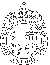
\includegraphics[width=2cm]{logo.pdf}
\vspace*{-2cm}

\hspace*{2cm}
 \begin{tabular}{l}
  {\ Pontificia Universidad Católica de Chile}\\
  {\ Escuela de Ingeniería}\\
  {\ IIC3695 Tópicos Avanzados en Inteligencia de Máquina 2019-1 }\\
  {\  }\\
 \end{tabular}
 \hfill
\vspace*{-0.2cm}
\begin{center}
{\Large\bf Entrega 1 Proyecto Semestral}\\
\vspace*{3mm}
{5 de julio de 2019}\\
\vspace*{1mm}
{\bf Raimundo Herrera - Manuel Vial }\\
\vspace*{1mm}
\end{center}
\hrule\vspace*{2pt}\hrule
%%%%%%%%%%%%%%%%%%%%%%%%%%
%%%%%%%%% ENCABEZADO %%%%%%%%%
%%%%%%%%%%%%%%%%%%%%%%%%%%
\thispagestyle{empty}

%\tableofcontents
%\newpage

%\thispagestyle{empty}
%\listoffigures
%\listoftables

%\newpage


\section{Introducción}
%Introducción: Se espera una buena motivación del problema para el lector, debe dar además una visión general del método/metodologíıa/etc., del aporte y de la estructura del documento.

%Contexto, propuesta y motivacion.
Existe un proyecto en ejecución de crianza de esturiones en Parral, región del Maule. Estos peces viven en piscinas que operan con un sistema llamado de recirculación, que permite reutilizar hasta un 95\% del agua luego de una limpieza de la misma con biofiltros.\\

Para el correcto crecimiento y desarrollo de los peces, se requiere mantener el agua en buenas condiciones, razón por la cual, ésta debe ser monitoreada constantemente. Para ello, se miden una serie de parámetros que indican de forma directa o indirecta si las condiciones son óptimas para los peces.\\

Algunos de estos parámetros deben mantenerse dentro de rango a toda costa, pues en caso contrario, la mortalidad puede ascender al orden de miles de peces. Tendría gran valor poder anticipar estos riesgos o mejor aún, evitarlos.\\

Luego de 5 años de crianza, se está analizando la posibilidad de realizar el monitoreo de parámetros de forma automática en vez de manual como se hace actualmente. Esto implica la compra y mantención de una serie de sensores de alto costo. Por ello, el estudio de relaciones entre parámetros se hace tentador para evitar gastos innecesarios.\\

Durante estos 5 años de operación, se han tomado datos de 6 parámetros, en todas las piscinas, tanto a la entrada del filtro biológico presente en las mismas, como en la salida, ambas mediciones tomadas una vez al día. Hay datos faltantes como se explicará más adelante y es esperable que también existan errores en las mediciones anotadas, pues se hacen de forma manual.\\

En la tabla [\ref{table:parameters}] incluida en los anexos, se muestran los principales parámetros medidos actualmente con sus rangos y valores óptimos. Con esos datos a disposición, uno de los resultados más valiosos que puede obtenerse, es la estimación de la concentración de nitrito en el agua, puesto que el sensor que lo mide es el más costoso.\\

En este trabajo se procede realizando una estimación de los parámetros que rigen la serie de tiempo asociada a la concentración de nitrito. Para ello, en primer lugar se realiza un análisis exploratorio y visual de los datos para tener una sensibilidad sobre el comportamiento de los mismos, las medidas de dispersión de las distintas variables, las correlaciones y autocorrelaciones de la mismas, junto con observar cada parámetro como una serie de tiempo, para ayudar visualmente a comprender el comportamiento de las curvas.\\

En segundo lugar, se trabaja con un modelo autorregresivo, particularmente con el llamado ARMA (\textit{Autoregressive Moving Average Models}), que intenta aprovechar la información pasada para calcular el valor presente de un parámetro. Sus coeficientes se calcularán con el método de Metrópolis-Hastings.

\section{Marco Teórico}
%Trabajos previos y/o Marco Teórico: Demuestran lo que leyó o estudió el alumno respecto al tema que está desarrollando. Además debe sentar las bases teóricas para el desarrollo del proyecto. En algunos casos podríıa definir gaps de conocimiento que se desean cubrir.

Luego de un análisis acabado de los datos fue posible constatar que usarlos como matriz de diseño no era un opción inteligente pues la autocorrelación es bastante alta y la naturaleza de los datos es altamente dependiente de la temporalidad. Así, lo más lógico es usar métodos que consideren esta relación intertemporal como las series de tiempo. Por ello, se entró a la investigación de modelos tipo ARMA o derivados.\\

Estos modelos intentan describir la dependencia de una variable buscada con las demás y consigo misma en tiempos pasados. En la mayoría de estos modelos se asume linealidad porque mantiene la simplicidad de las operaciones y no pierde mucho en capacidad de descripción de las realidades que busca predecir.\\

En términos de ecuaciones, se puede escribir el modelo ARMA como sigue:

\begin{equation*}
    y_{t} = \sum_{i=1}^{p}{a_{i} y_{t-i}} + \sum_{i=1}^{q}{\sum_{j=1}^{M} c_{i}^{j}u_{t-i}^{j}} + \epsilon_{t}
\end{equation*}
\\

En este modelo, se reciben entradas $u$ que, junto a los valores anteriores de $y$ y el error $\epsilon$ definen cuál va a ser el nuevo valor para $y$. Las entradas $u$ corresponden a aquellos parámetros que se consideran como causas directas del valor a predecir $y$. Por otro lado, $p$ y $q$ expresan cuántas muestras anteriores se toman del propio $y$ y de las entradas, respectivamente. Los subíndices indican temporalidad (en general, discreta), y los supraíndices indican a qué entrada corresponde, pues puede haber más de una. Los coeficientes $a$ y $c$ son los que permiten ajustar el modelo. $M$ corresponde a la cantidad de parámetros que se utilizarán como entrada. En la siguiente sección se explica con más detalle el modelo ARMA. \\

Los modelos de este tipo son ampliamente usados en la literatura y la industria porque permiten explicar bastante bien la realidad en muchos casos, manteniendo una forma matemática simple y fácil de manejar. Así, existe mucha investigación que relaciona estos modelos con distintos rubros y ocupa técnicas de distintas ramas del conocimiento \cite{arma1}. La búsqueda de los coeficientes usando \textit{maximum likelihood} se ocupa desde hace más de 10 años \cite{arma2}.\\

En este proyecto, se busca predecir el nivel de nitritos. Para ello, como no conviene aumentar demasiado la cantidad de parámetros, se consideran algunos como entrada $u$ y se supone que los demás generan un efecto poco considerable por lo que no se distinguen del ruido o error. La elección de cuáles parámetros se consideran y cuáles no es crucial para los resultados del modelo, por lo que en las secciones venideras se discutirá sobre las distintas elecciones, y su influencia en el rendimiento de la predicción. El modelo asume que existe ruido \textit{gaussiano}.\\

Se busca encontrar los coeficientes de $a_{i}$ y $c_{i}^{j}$ para cada j y cada i. La forma en este caso, será la maximización de la \textit{likelihood}. La literatura muestra que métodos como Gibbs-Sampling o su versión general, Metrópolis-Hastings pueden ser ocupados para esto \cite{arma-gibbs}. En este caso, se usó Metrópolis-Hastings para obtener los coeficientes, pero se mantiene abierta la posibilidad de probar con Gibbs-Sampling para comparar resultados.\\

Un elemento a analizar es la estructura de los datos faltantes. Existen 3 mecanismos que la explican, \textit{Missing Not At Random (MNAR)}, \textit{Missing At Random (MAR)} y \textit{Missing Completely At Random (MCAR)} \cite{mcnar}. Para el conjunto de datos utilizado, se considera que la información faltante se rige bajo \textit{MAR}. Lo anterior, si bien no se puede probar sin acceso a la información faltante, se deduce a partir de que la falta de datos no se relaciona con el valor de los datos ausentes, sino que con el valor de otras variables observadas \cite{mcnar}. Según la información entregada por la planta, existen situaciones relacionadas con la operación que determinan que ciertos días en específico no se realicen mediciones. De este modo, como sí existe información observable que da cuenta de la falta de datos, se descarta que sea \textit{MCAR}, y puesto que no depende de los valores de los datos que faltan sino de otras variables observadas, se descarta que sea \textit{MNAR} \cite{mcnar}.\\

Cuando se concluye que la información es \textit{MAR} o \textit{MCAR} se puede proceder ignorándola para el análisis posterior. No obstante, si bien es un análisis relevante de hacer, se ha mostrado que si la suposición de \textit{MAR} es incorrecta, dado que no se puede probar, esto no distorsiona significativamente las estimaciones \cite{mcnar}, por lo que asumirlo no implica un riesgo mayor para el modelo.

% La posibilidad de completar datos faltantes en la base de datos sigue vigente porque las filas que presentan la totalidad de sus datos son en realidad menos de un tercio del total de datos. Así, los métodos gráficos u otros surgen como alternativa atractiva para aumentar la información disponible para encontrar los coeficientes.

%Por otra parte, para la predicción usaremos procesos de regresión gaussianos. Intentaremos reconocer ciclos con modelos autoregresivos sobre la variable más importante, utilizando los demás como perturbaciones e intentando encontrar los parámetros con métodos como el de Metropolis-Hastings.

\section{Metodología}
%Metodologíıa: Explica lo que se desarrolló y cómo se desarrollo.

Como se mencionó anteriormente, la primera parte del trabajo desarrollado consistió en un análisis exploratorio de los datos, con el objetivo de entender el comportamiento de los mismos.

\subsection{Visualizaciones}

En primer lugar, para observar si existen distribuciones que rigen a cada parámetro, se dispusieron histogramas, junto con una distribución normal de acuerdo a la media y desviación estándar de cada uno a modo de referencia. En la figura [\ref{fig:histograms1}] se muestran dos de los histogramas más importantes -los más correlacionados- el de nitrito y el de nitrato, junto con el ajuste normal. Como se observa, los datos están lejos de distribuir de acuerdo a una distribución normal. Si bien muestran ciertas similitudes en su forma, la correlación, como se mostrará más adelante no es alta.\\

\begin{figure}
  \centering
    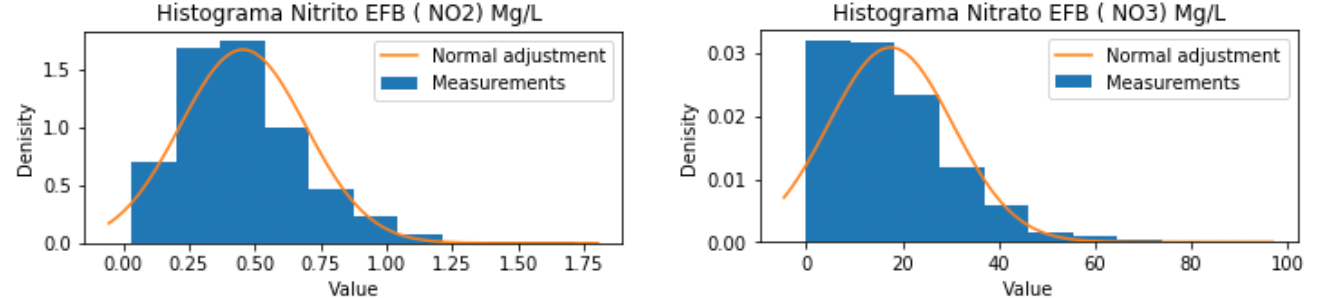
\includegraphics[width=0.75\textwidth]{img/histograms1.png}
  \caption{Histograma para mediciones de nitrito y nitrato}
  \label{fig:histograms1}
\end{figure}

En segundo lugar, se visualizaron los parámetros como series de tiempo, lo que es de especial interés dado el modelo a utilizar. Las visualizaciones de dos de las más notables se muestran en los anexos [\ref{fig:timeseries2}], sin embargo, como no aportaban mucho, se optó por mostrar series de acuerdo a promedios de las mediciones en un mes, como se ve en la imagen [\ref{fig:timeseries1}], además de las por día, para observar si existían comportamientos a una escala temporal mayor que no se apreciaban con el ruido diario. Si bien esta visualización otorga cierta información respecto a \textit{peaks} compartidos, no es suficiente para argumentar una similitud directa.

\begin{figure}[H]
  \centering
    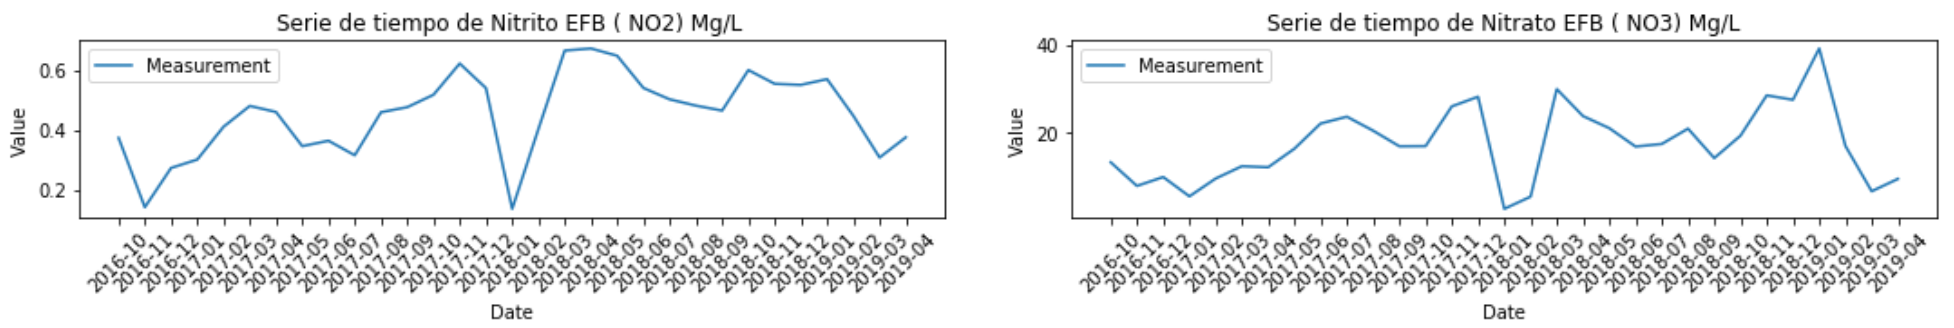
\includegraphics[width=0.95\textwidth]{img/timeseries1.png}
  \caption{Series de tiempo promediadas por mes para las mediciones de nitrito y nitrato}
  \label{fig:timeseries1}
\end{figure}

\subsection{Correlaciones}
En el análisis de la correlación se encontraron parámetros relacionados entre sí, que confirmaron algunas hipótesis sobre el comportamiento de ciertos compuestos químicos. Por ejemplo, por su composición, el nitrito y nitrato deben estar íntimamente relacionados.\\

En la matriz de correlaciones mostrada en los anexos [\ref{fig:corrmatrix1}] se observa que, si bien ninguna correlación es superior a 0.5, existen ciertos pares de datos que definitivamente no se correlacionan y otros que tienen cierta cercanía.\\

Tras lo anterior, surge naturalmente la necesidad de observar las correlaciones temporales de un mismo parámetro. Con eso en mente, se despliegan en la figura [\ref{fig:autocorr}] las autocorrelaciones de los parámetros considerando desplazamientos temporales de hasta 10 días. Ahí se aprecia de modo más evidente que los parámetros tienen alta autocorrelación y que por lo tanto la temporalidad no puede ser ignorada, siendo propicio para esto el modelo escogido.\\

\begin{figure}[H]
  \centering
    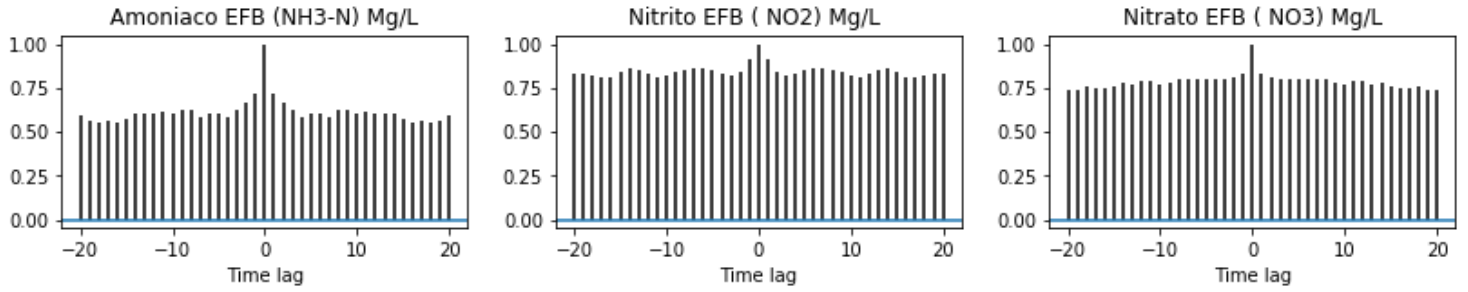
\includegraphics[width=0.85\textwidth]{img/autocorr.png}
  \caption{Autocorrelación para las mediciones de amoniaco, nitrito y nitrato}
  \label{fig:autocorr}
\end{figure}

Por otro lado, una opción interesante es desagregar la información contenida en la correlaciones entre 2 parámetros. Esto se puede lograr controlando por una tercera variable, fijando un rango por ejemplo. Existía la hipótesis de que a ciertas temperaturas, los valores de nitrito y nitrato se relacionaban fuertemente. Esto se pudo comprobar al ver que en el rango de los 23º a 24º, la correlación es de 0.8, muy por sobre el 0.5 reportado originalmente sin considerar la temperatura. Esto da luces de que efectivamente existe una mayor correlación entre la concentración de ambos compuestos, pero que es difícil de apreciar si se consideran rangos amplios de temperatura. Resultados similares ocurren con el pH, donde ciertos intervalos aumentan la correlación.

\subsection{Descripción de los datos}

Por último, una descripción de los datos desde el punto de vista de las medidas estadísticas comunes, entrega que las medias, mínimos y máximos de los datos medidos en las piscinas, están acordes a los rangos esperados. Sin embargo, muestran que existe en ciertas mediciones una desviación muy alta, como es el caso del nitrato, donde para una media de 17.6 mg/L en una de las piscinas, se obtuvo una desviación estándar de 12.9. Lo anterior puede anticipar la gran variación que puede tener nuestro modelo a la hora de predecir, lo que sugiere la necesidad de más y mejores mediciones para poder predecir con certeza los valores esperados.

\subsection{ARMA}

El modelo ARMA consta de tres elementos que permiten predecir una variable: autorregresión, ventana móvil y error. Cada uno aporta de una forma particular a obtener resultados que pueden ser muy cercanos a la realidad en muchos casos.\\

La autorregresión se refiere al efecto inercial de la propia variable, indica en qué medida tiende a mantenerse estable, cuánto afectan sus valores anteriores en el presente.\\

La ventana móvil, asume que el efecto que realizan las entradas en el valor actual de $y$ se realiza de dos formas: influyendo sobre valores pasados de la propia variable $y$, y también de forma directa sobre su valor actual. Este efecto, se considera por un cierto período en el tiempo, a esto se le llama ventana móvil. En este caso se entiende que las entradas son algunos de las otras variables medidas.\\

Por último, se incluye un término de error para asumir que pueden existir perturbaciones no consideradas en el modelo, que lo hacen diferir de la realidad. Aquí se agrupa el efecto de las variables no introducidas y también de otras cuyos datos no se consideran, como por ejemplo, la cantidad de peces o el nivel de recambio del agua.\\

Los usos que se le pueden dar a modelos tipo ARMA son muy variados, áreas de predicción y control los ocupan de forma continua. En este último ámbito, se suelen usar las entradas para modelar aquello que se puede manejar, y agrupar los términos restantes en el error o en otros términos separados. Esto tiene sentido porque lo que se intenta es definir ese vector de control que permitirá manejar la salida. En casos de predicción, la separación se hace de forma distinta puesto que no hay entradas. Aquí, cobra sentido la idea de separar las variables que afectan de forma directa y en mayor medida en la salida, para considerar que las restantes no son más que ruido o un error pequeño, no modelado en detalle.\\

El modelo ARMA se implementó con los siguientes valores para los parámetros mencionados anteriormente: $p = 2$, $q = 3$, $M = 2$, $\epsilon$: $\mathcal{N}(0, 1.3)$. Los parámetros recién mencionados y las tres mediciones que se usaron como entrada, se obtuvieron iterando con distintos números y conjuntos de variables para ver cuál tenía mejores resultados. \\

Para obtener la \textit{likelihood} de los parámetros, se asumió independencia y se obtuvo la probabilidad del dato real de nitrito, dada la estimación realizada a partir de cada conjunto de datos.

\subsection{Metrópolis-Hastings}

Luego, se ocupó el método de muestreo Metrópolis-Hastings para la obtención de \textit{sets} de coeficientes para ARMA. Esto se realizó utilizando como \textit{jumpling distribution} una gaussiana centrada en la muestra anterior (una para cada coeficiente) y con una desviación estándar alta para lograr que recorra bien el espacio de posibles coeficientes. Como $p$ se usó directamente la log-likelihood de ARMA, ya comentada. El \textit{alpha} usado para aceptar la muestra fue el siguiente:

\begin{equation*}
    \alpha = min(exp(p^*(x^*) + q(x_{t}\mid x^*) - p^*(x_{t}) + q(x^*\mid x_{t})), 1)
\end{equation*}


\section{Resultados y análisis}
%Resultados y análisis: Presenta (tablas, gráficos, etc.) los resultados de la metodologíıa y describe con un juicio crítico lo que se obtiene.

Se muestran algunos gráficos que comparan la predicción realizada con los valores reales. Hay diferencias muy significativas en la decisión de qué entradas usar o qué parámetros elegir para el modelo ARMA.\\

Fue posible hallar dos combinaciones de parámetros y entradas que logra predecir de manera bastante certera el valor de los nitritos. Es cierto que el ajuste no es perfecto ni modela cada subida o bajada, pero si muestra un buen seguimiento de tendencias que es de gran importancia. De hecho, un seguimiento más cercano podría ser muestra de un sobre ajuste.

%%%%%%%%%%%%% cambiar figuras
\begin{figure}[H]
  \centering
    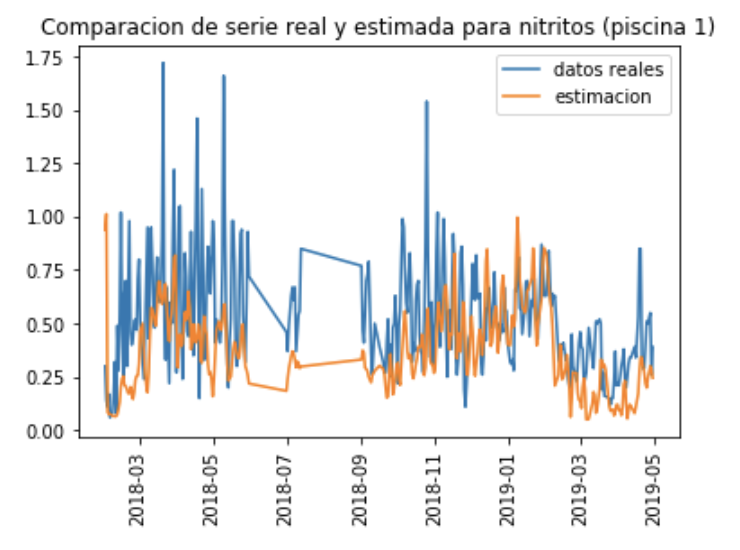
\includegraphics[width=0.4\textwidth]{img/nitrato-temp.png}
    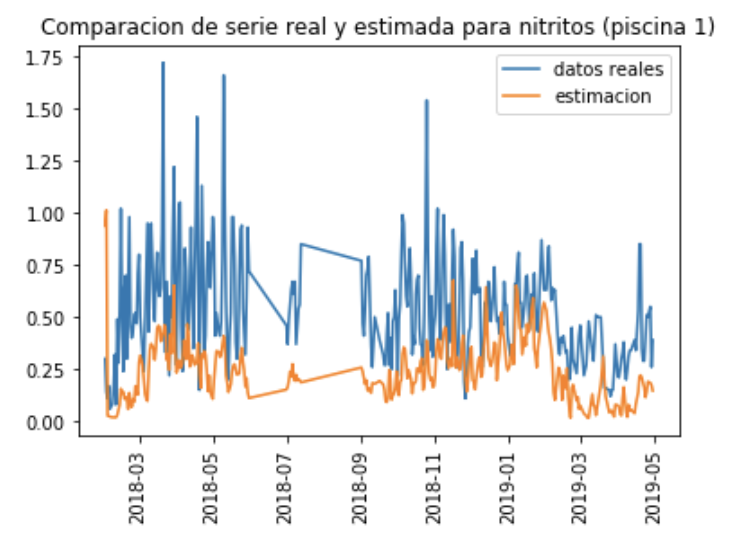
\includegraphics[width=0.4\textwidth]{img/nitrato-ph.png}
  \caption{Serie estimada usando nitrato y temperatura (izquierda), nitrato y pH (derecha)}
  \label{fig:results}
\end{figure}

Las mejores predicciones se obtuvieron usando como entrada dos datos anteriores de nitritos, y tres datos anteriores de temperatura y nitrato.\\

La inclusión de más información en tiempo o más variables provoca una complejización del problema que afecta en la calidad de los resultados de la predicción. En los anexos [\ref{fig:res_malo}] se muestra un ejemplo de ello, en que se usaron 5 períodos y se consideran 5 entradas.\\

Sería prudente realizar un estudio más profundo de la química que opera en las piscinas, para entender cómo es la relación intertemporal entre parámetros. Esto permitiría darle adecuados parámetros iniciales al modelo para que luego itere perfeccionándolos. Además, daría luces de formas de combinación de parámetros no consideradas aquí o sobre la necesidad de incluir algún grado de no linealidad.\\

Por otro lado, la hipótesis de que la correlación entre los parámetros es relevante, pero lo es aún más si se consideran correlaciones con otros parámetros fijos, se comprueba. Se realizó el mismo experimento, con otro parámetro altamente correlacionado al nitrito, el amonio, pero que no presenta una correlación mayor a temperaturas controladas. Los resultados para ese parámetro fueron muy lejanos a los buenos resultados obtenidos anteriormente, lo que comprueba la relevancia de esa información, como se muestra en el anexo [\ref{fig:results-amonio}].

\section{Conclusiones}
%Conclusiones: Resalta los principales hallazgos del proyecto (lo bueno y lo malo), además proyecta posibles mejoras o variantes del trabajo realizado.

En el presente proyecto se planteó la posibilidad de predecir el valor de los nitritos en piscinas acuícolas a partir de datos pasados y de otras variables más fáciles de medir. Para ello fue necesario hacer un análisis de los datos que permitiera entender a grandes rasgos las principales características de comportamiento y relaciones existentes entre las variables. Luego, fue posible plantear un modelo que tomara en cuenta los hallazgos y luego definir los detalles del mismo.\\

El estudio de los datos sirvió para entender qué experimentos tiene sentido hacer y cuáles no, qué metodologías pueden aportar información relevante y cuales no son adecuadas para este tipo de datos. Se optó por las metodologías que consideran la temporalidad de los datos \textit{versus} las que los toman como mediciones independientes.\\

%Se comprendió que la correlación entre datos de entrada y salida del filtro biológico (las primeras 5 columnas y las siguientes 5) es muy alta, razón que no permite asumir su independencia para aumentar los datos sin más trabajo.\\

Por otro lado, se observó que un análisis exploratorio inicial aporta perspectivas sobre la estructura de los datos, pero que existen relaciones intrínsecas de los mismos que pueden aparecer al estudiarlos más detenidamente, como es la correlación entre variables fijando otras. También que un buen análisis permite escoger parámetros adecuados que tienen una alta incidencia en los resultados.\\

Se pudo ejecutar una rutina de Metrópolis-Hastings que opera buscando parámetros para el modelo ARMA propuesto. Se obtuvieron resultados en un principio lejanos a la realidad pero que luego con un análisis detenido de los datos se ajustaron mucho más, llegando a obtener series de tiempo bastante ajustadas a la real, que pueden servir de referencia a la hora de predecir datos futuros.\\

El método propuesto resultó ser sumamente sensible a las correlaciones entre los datos y a la temporalidad, como se había teorizado en un principio. De este modo, la comprensión de los datos fue fundamental para escoger el modelo, seleccionar los parámetros, y finalmente decidir qué experimentos realizar.\\

Inclusión de estudios químicos sobre las relaciones entre varias, o la temporalidad de los efectos entre una y otra podrían aportar de forma significativa a idear modelos que capten mejor la realidad. De igual forma, un aumento de los datos podría significar un crecimiento en robustez de los resultados que pueden verse como pasos a seguir con miras a alcanzar resultados útiles para la empresa.\\


Por último señalar que con pocos datos, técnicas relativamente sencillas y algoritmos sumamente estudiados, se logró aplicar lo aprendido a un problema real como es predecir el nivel de nitritos en una planta de crianza de esturiones, lo que puede significar grandes ahorros de costos para el proyecto en cuestión.

%pero que muestran un código operativo al que le falta ajustarse y operar por más tiempo para acercarse a la realidad. \\

% El mayor avance es en realidad la comprensión de una metodología conjunta que permite lograr predicciones y la programación de una versión básica de esta. Con eso, ya es posible ir perfeccionando la técnica, agregando más datos y robusteciendo el método para lograr resultados útiles.\\


\newpage
\begin{thebibliography}{3} %% Donde hay un 3, indicar el número de elementos que tendrá la bibliografía

%Bibliografía: Utiliza un formato estandarizado para referenciar todos los documentos utilizados para el desarrollo del proyecto.

%% ¿Cómo se usa \bibitem{alias}? Donde dice alias, poner un sobrenombre al documento que después se puede usar a lo largo del texto para hacer referencia a éste.
%% Para citar, hacer \cite{alias}
%% \bibitem{nunez}F.~Nuñez, \emph{Experiencia 2: Identificación y LoopShaping}. Laboratorio de Control Automático IEE2683, Pontificia Universidad Católica de Chile, 2018.

\bibitem{arma1}Ling, Zhu, and Yee. "Diagnostic Checking for Non-stationary ARMA Models with an Application to Financial Data." North American Journal of Economics and Finance 26.C (2013): 624-39. Web.

\bibitem{arma2}Mcleod, and Zhang. "Faster ARMA Maximum Likelihood Estimation." Computational Statistics and Data Analysis 52.4 (2008): 2166-176. Web.

\bibitem{arma-gibbs}Ravishanker, Nalini, and Bonnie Ray. "Bayesian Analysis of Vector ARMA Models Using Gibbs Sampling." Journal of Forecasting 16.3 (1997): 177-94. Web.

\bibitem{mcnar}Dong and Peng. "Principled missing data methods for researchers". SpringerPlus 2.1 (2013): 222. Web.

\end{thebibliography}

\newpage
\section*{Anexos}

Se incluyen 2 cuadernillos (\textit{jupyter notebooks}) a modo de anexo con el análisis de los datos, y el modelo junto con su implementación. \\

El análisis de datos presente en \texttt{EDA.ipynb} incluye:
\begin{itemize}
    \item Histogramas para todos los parámetros de la piscina 1.
    \item Histogramas con ajuste normal.
    \item Series de tiempo de todos los parámetros.
    \item Series de tiempo promediadas por mes.
    \item Matriz de correlaciones.
    \item Gráficos de parámetro \textit{vs} parámetro que muestran correlación.
    \item Gráficos de autocorrelación para todos los parámetros.
    \item Descripción de los datos.
    \item Análisis de correlación de 3 parámetros
    \item Exploración respecto al mecanismo de \textit{missing data}.\\
\end{itemize}

Parte del desarollo del modelo se incluye en \texttt{modelo1.pdf} y \texttt{modelo2.pdf} que incluyen distintas iteraciones del código utilizado para ARMA, Metropolis-Hastings, algunas visualizaciones, entre otros.\\

\centering
\begin{table}[H]
\begin{tabular}{|l|c|c|c|c|}
\hline
\textbf{Parámetro} & \textbf{Unidad} & \textbf{Rango Equipo} & \textbf{Rango Cultivo} & \textbf{Óptimo} \\ \hline \hline
Temperatura & \textordmasculine Celsius & 0 a 30 & 8 a 25 & 20 \\ \hline
Amonio ($NH_{4}$) & mg/L & 0 a 300 & \textless 3 & \textless 3 \\ \hline
Amoniaco ($NH_{3}$) & mg/L & 0 a 300 & \textless 1 & \textless 1 \\ \hline
Nitrito ($NO_{2}$) & mg/L & 0 a 1.15 & \textless{}3 & \textless{}3 \\ \hline
Nitrato ($NO_{3}$) & mg/L & 0 a 100 & 70 & 70 \\ \hline
pH & Unidad & 0 a 14 & 7 a 8 & 7 \\ \hline
\end{tabular}
\caption{Parámetros del agua con unidades y rangos}
\label{table:parameters}
\end{table}

\begin{figure}
  \centering
    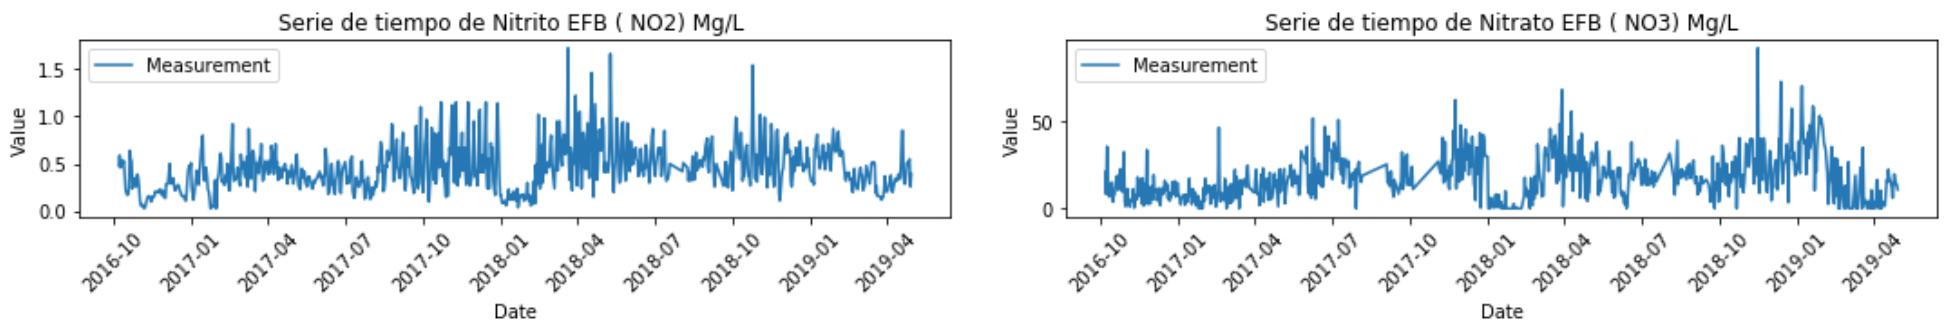
\includegraphics[width=0.95\textwidth]{img/timeseries2.png}
  \caption{Series de tiempo diarias para las mediciones de nitrito y nitrato}
  \label{fig:timeseries2}
\end{figure}

\begin{figure}
  \centering
    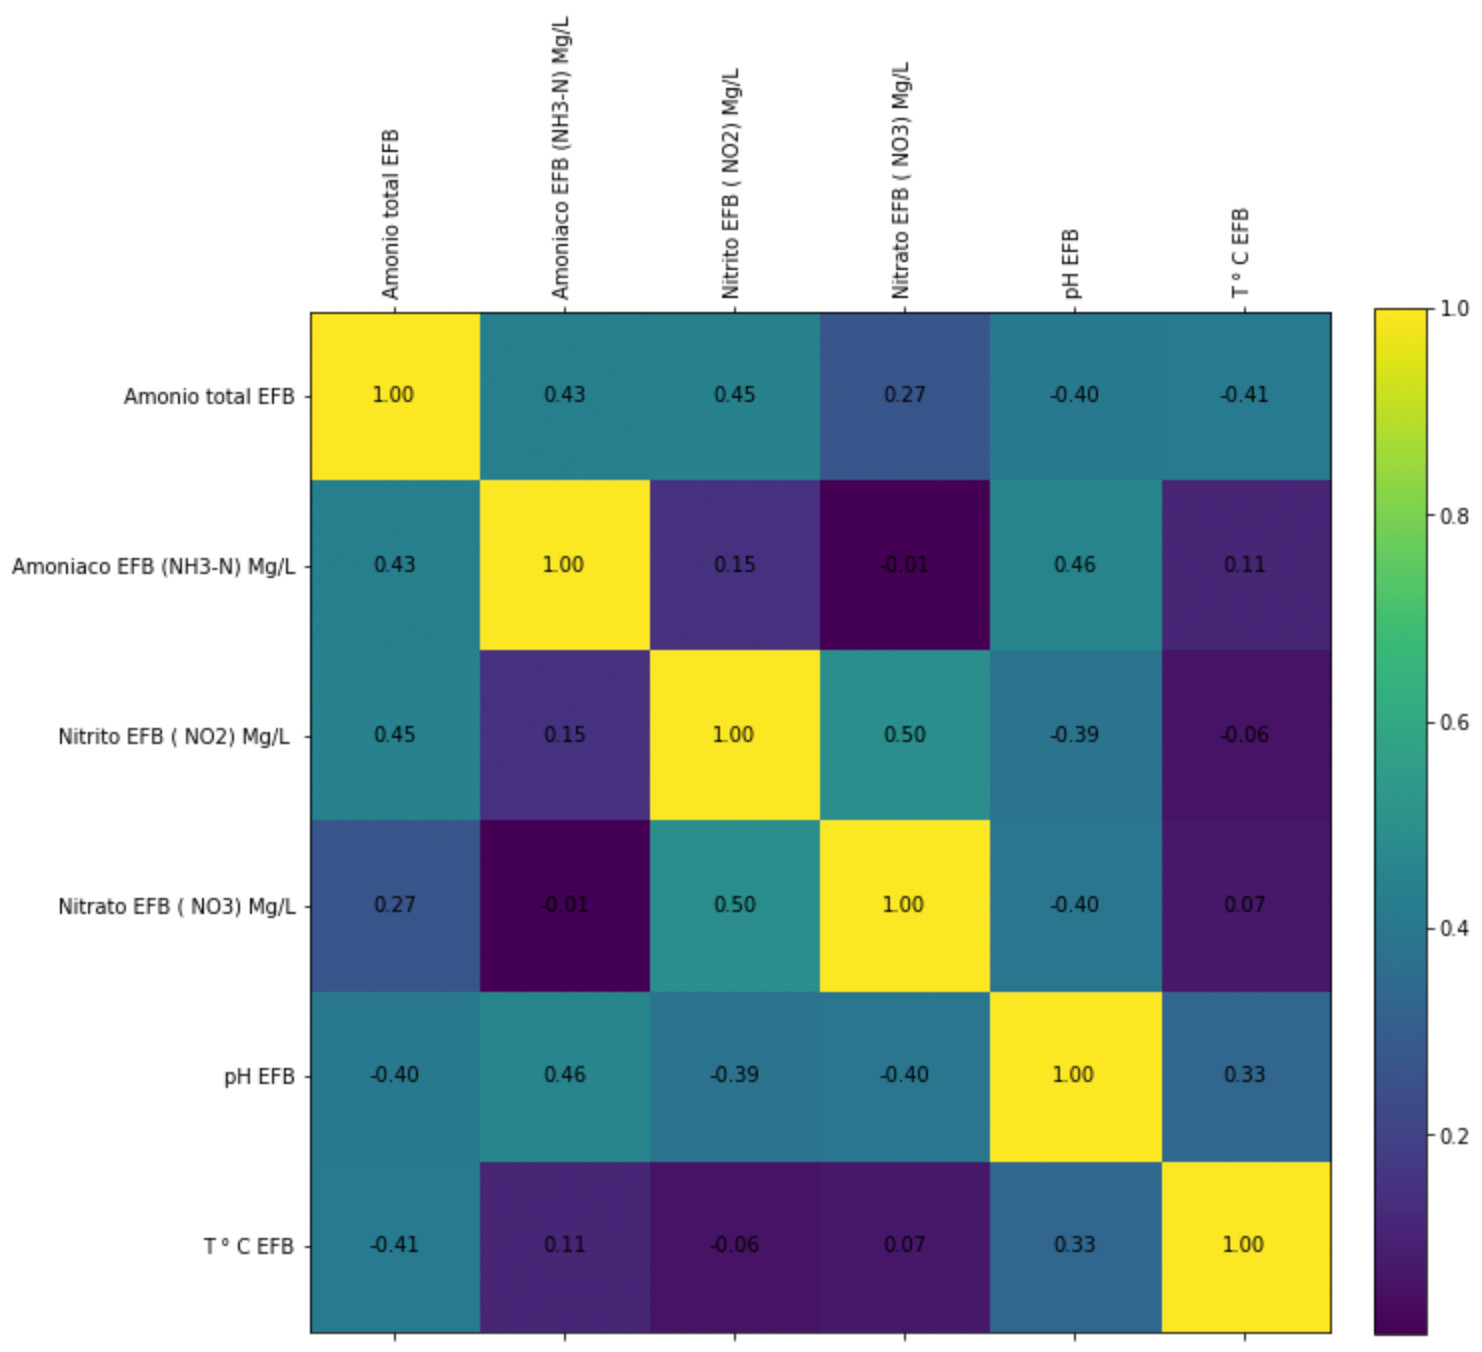
\includegraphics[width=0.8\textwidth]{img/corrmatrix1.png}
  \caption{Matriz de correlaciones entre parámetros}
  \label{fig:corrmatrix1}
\end{figure}


\begin{figure}
  \centering
    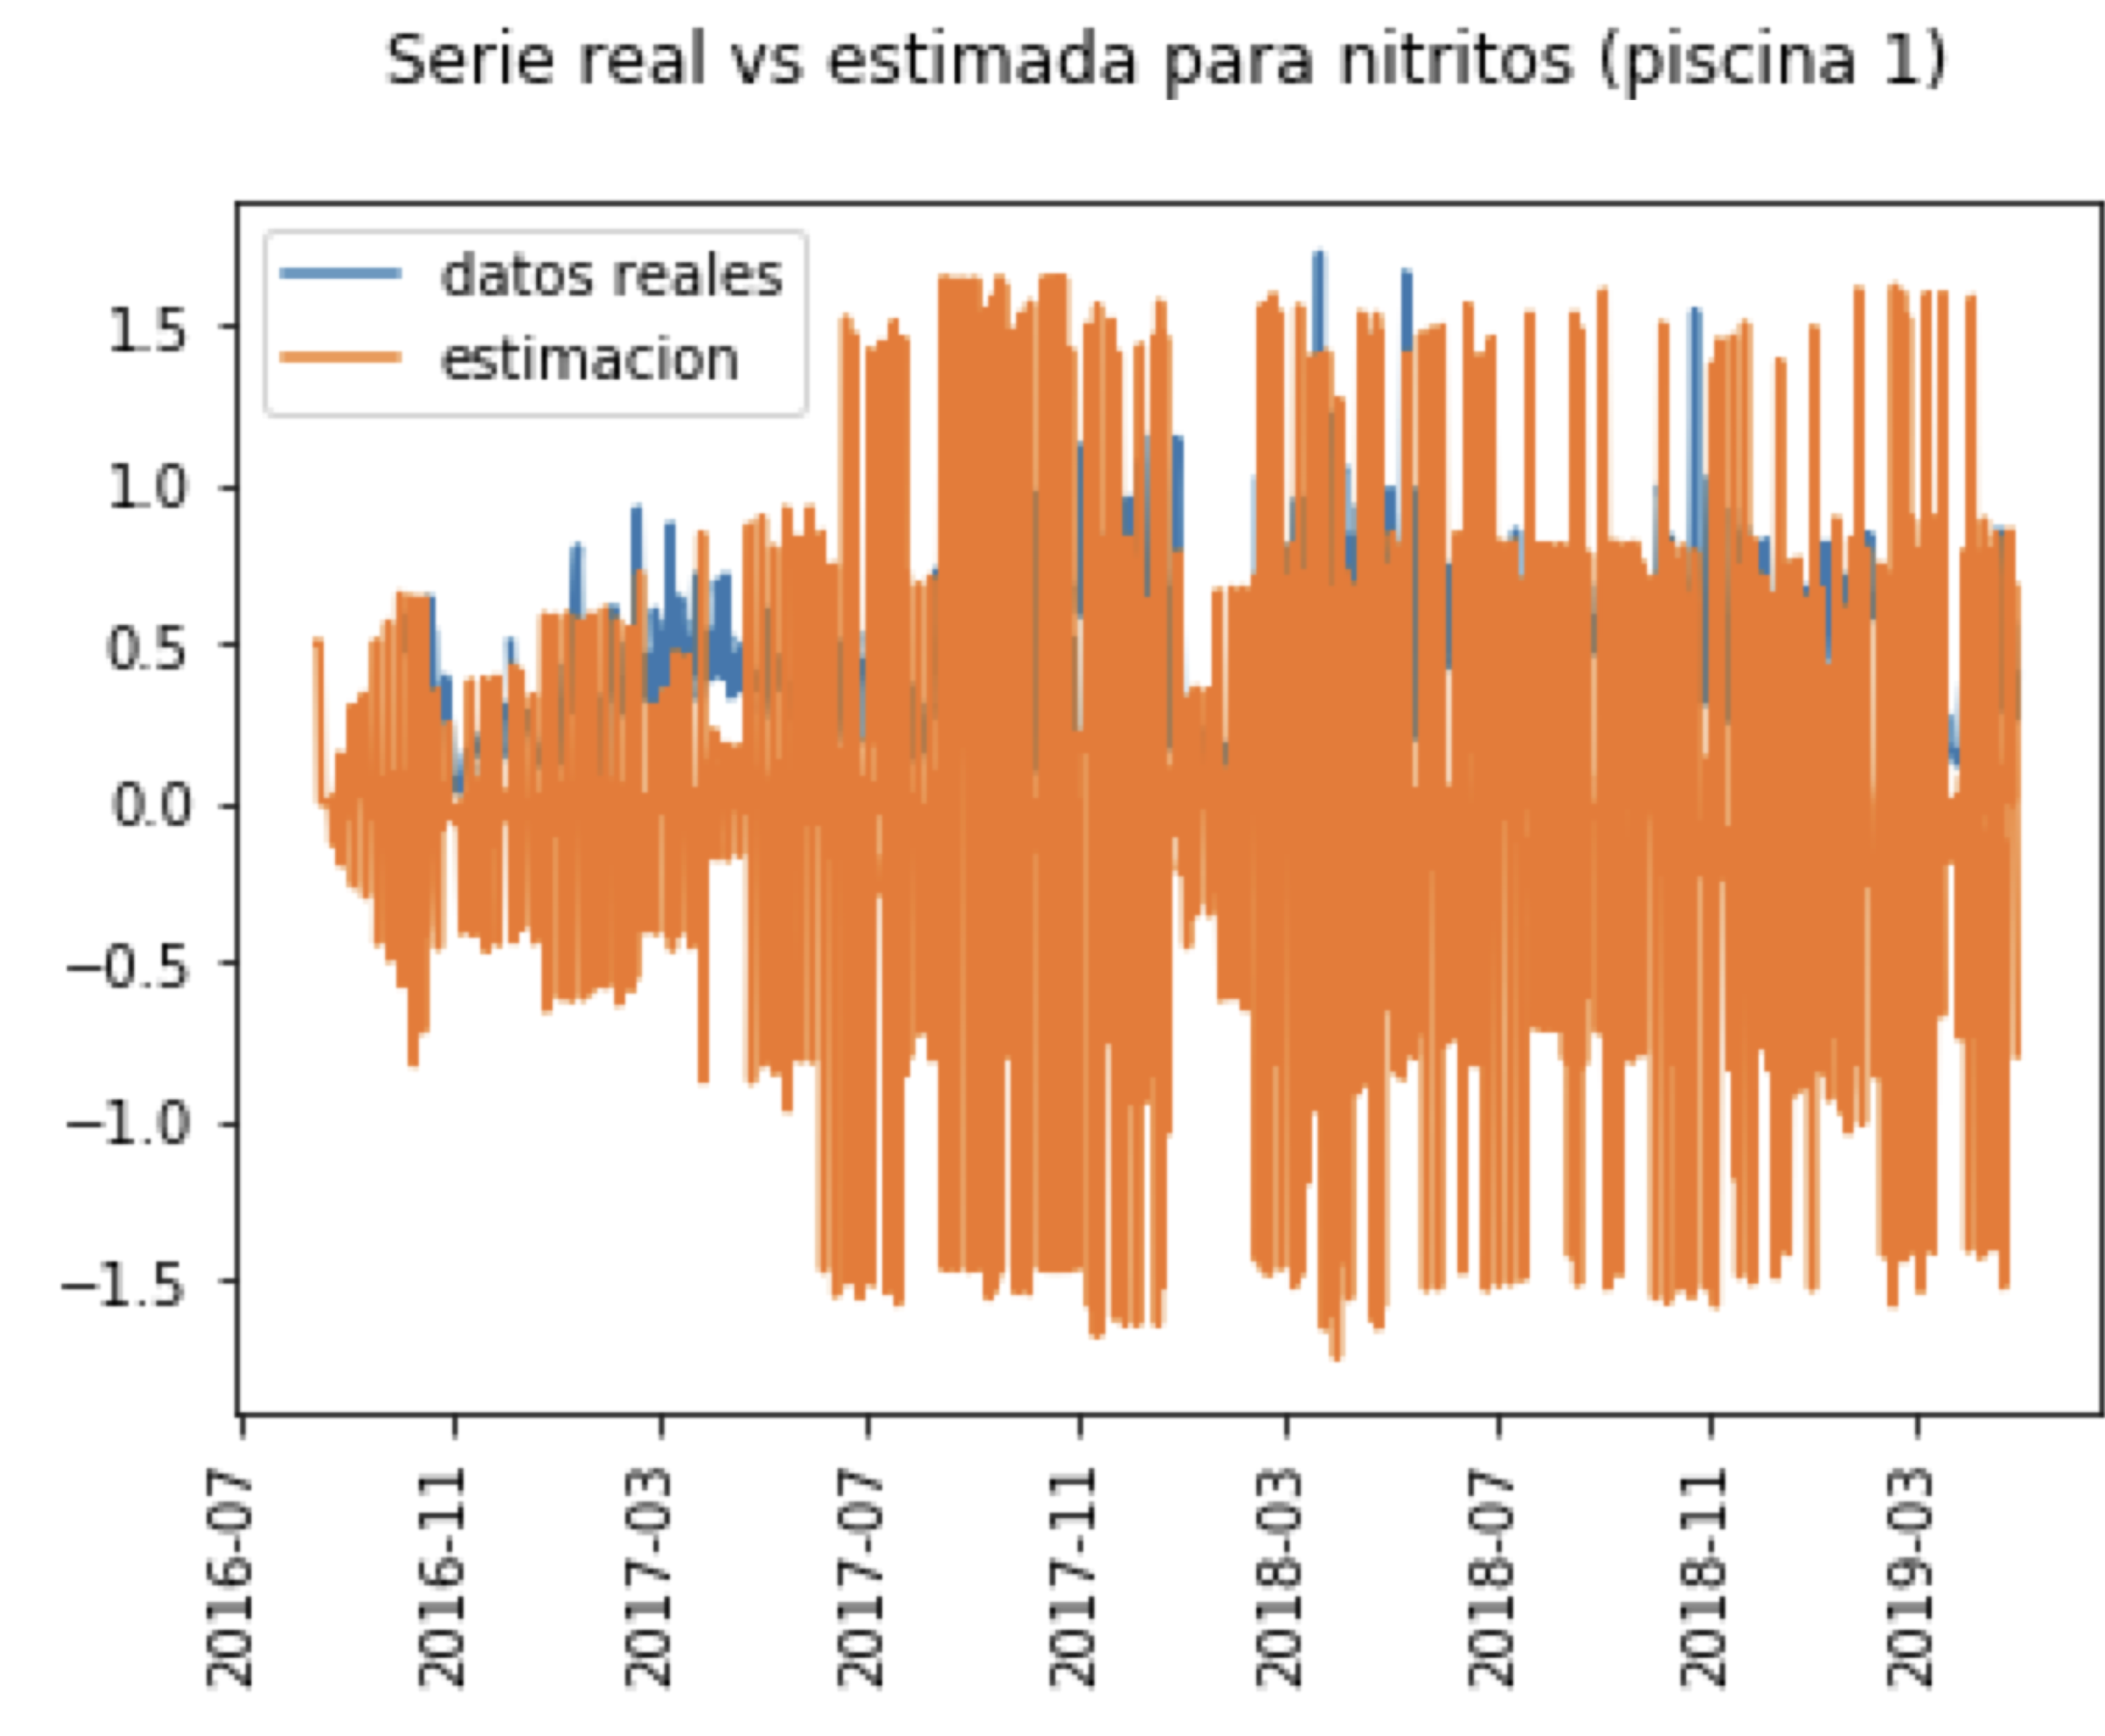
\includegraphics[width=0.4\textwidth]{img/res_malo.png}
  \caption{Resultados para la serie de tiempo predicha con exceso de parámetros.}
  \label{fig:res_malo}
\end{figure}

\begin{figure}
  \centering
    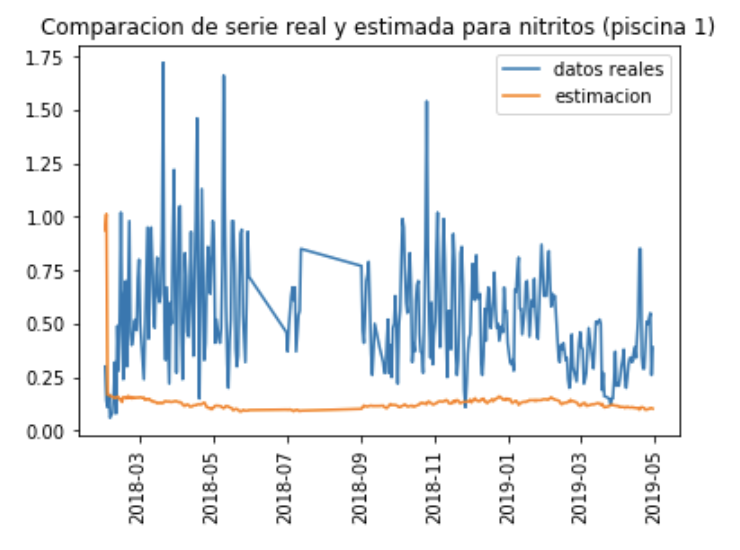
\includegraphics[width=0.4\textwidth]{img/amonio-temp.png}
  \caption{Resultados para la serie de tiempo con amonio y temperatura.}
  \label{fig:results-amonio}
\end{figure}

%\section{Hojas de datos}
%\includepdf[pages=-]{Hoja_datos.pdf}

\end{document}

% \begin{figure}[H]
%      \centering
%      \includegraphics{}
%      \caption{``Ir y Venir'' con control P: comparación con experimento sin control}
%      \label{fig:iv_p_2}
%  \end{figure}{}